\documentclass[10pt,twocolumn]{article}

\usepackage{listings}
\usepackage[utf8]{inputenc}
\usepackage[T1]{fontenc}
\usepackage{graphicx}
\usepackage{hyperref}
\usepackage{amsmath}
\usepackage{algorithm}
\usepackage{algpseudocode}
\usepackage{booktabs}
\usepackage{microtype}
\usepackage[margin=1in]{geometry}

\lstset{
  language=HTML,
  basicstyle=\ttfamily\small,
  breaklines=true,
  frame=single
}

\begin{document}

\title{Mini-ARC: Solving Abstraction and Reasoning Puzzles with Small
Transformer Models}

\author{Paul Fletcher-Hill}
\date{November 12, 2024}

\maketitle

\begin{figure*}[h!]
  \centering
  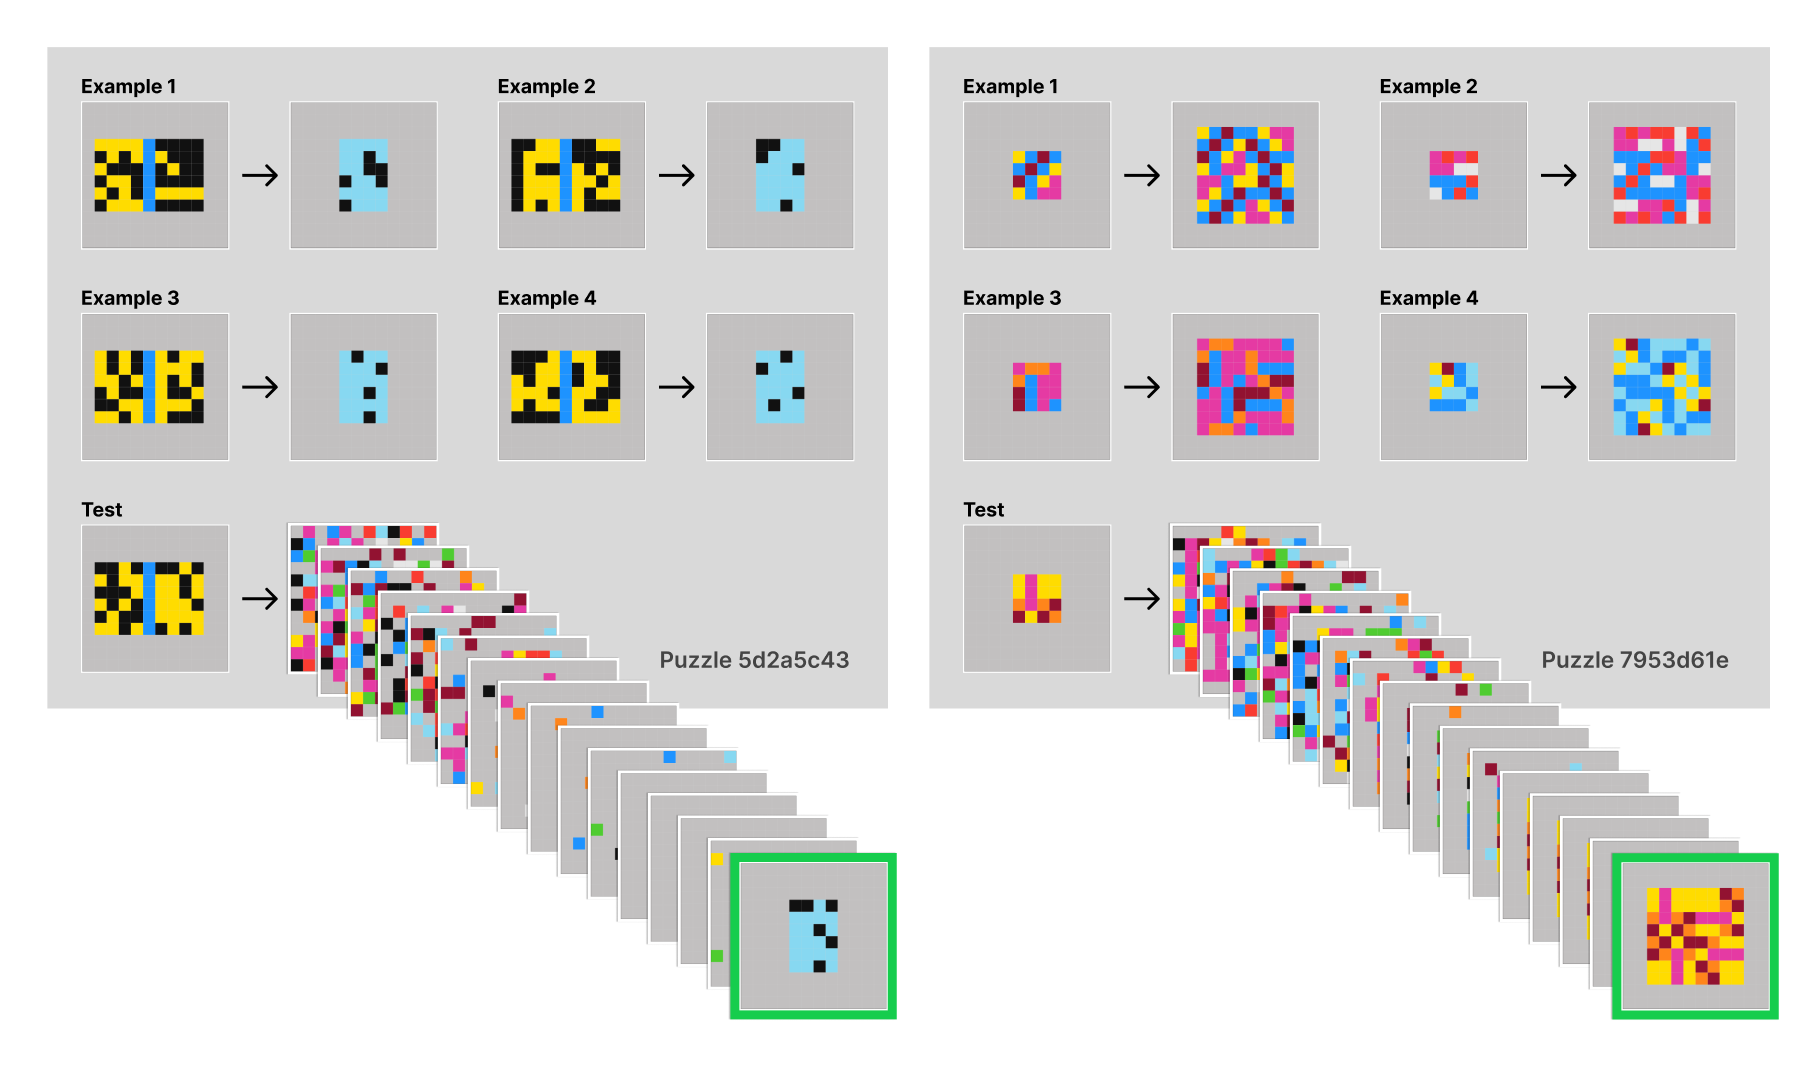
\includegraphics[width=\textwidth]{figures/header.png}
  \caption{Mini-ARC solves ARC puzzles using customized small
    Transformer models. These are real predicted outputs for two ARC
  puzzles as they progress through the Transformer encoder layers.}
  \label{fig:top-image}
\end{figure*}

\begin{abstract}
  The Abstraction and Reasoning Corpus (ARC)\cite{arc} is a benchmark
  to test the ability of artificial systems to adapt, learn on the
  fly, and quickly acquire new skills in a human-like way. The
  benchmark has proven challenging for even the most advanced
  language models to solve. In this paper, I explain a novel approach
  to solving ARC puzzles that uses (1) small (67M param) Transformer models
  trained exclusively on ARC puzzles, (2) test-time training (TTT),
  and (3) refinement. I demonstrate that a system combining these
  three strategies is able to solve 41\% of puzzles from a subset of
  the public ARC evaluation dataset that fit the model dimensions.
  This result is notable because
  it is achieved with a very small model and without the use of
  search, language models, or program synthesis.

  Code is available at: \url{https://github.com/pfletcherhill/mini-arc}
\end{abstract}

\section{Introduction}

\subsection{The Abstraction and Reasoning Corpus (ARC)}
The Abstraction and Reasoning Corpus (ARC)\cite{arc} is a benchmark published
in 2019 by Francois Chollet which aims to test models' ability to
reason and efficiently learn new patterns. The benchmark is composed
of 2D puzzles that are relatively simple for humans to solve but
which have stumped even the most advanced LLMs.

ARC puzzles are structured as a list of
input/output grids, each of which demonstrate some sort of
transformation. The goal is to infer the transformation from the list
of input/output grids and then apply the same transformation to a new
input grid. The benchmark is very diverse in terms of the
transformations, including concepts like counting, gravity, rotation, and more.

The ARC Prize\cite{arcprize2024} is a competition to build an
artificial system that solves not-seen-before ARC puzzles. There are
800 publicly available ARC puzzles (400 easy ones and 400 hard ones),
but the competition evaluates each submission against 100 secret
puzzles that may or may not share concepts with the publicly available puzzles.

Many of the most successful systems thus far have made use of
fine-tuned LLMs and a combination of test-time training and program
synthesis to try to solve puzzles. Two teams recently beat 50\% on
the 2024 ARC Prize leaderboard using similar approaches.

\subsection{Motivation}
While considerable progress is being made with the approaches
described above, I wanted to see if similar performance could be achieved
without using language models at all. Intuitively, I do not "think"
in terms of language when solving ARC puzzles myself, so I wondered
whether an artificial system could reason and identify patterns
without language too.

\section{Related Work}

\subsection{Test-Time Training (TTT)}
Test-time training (TTT) is a meta learning strategy being used by
multiple groups to quickly adapt pre-trained models for new puzzles
when they see them. MindsAI, the group currently holding the top spot
on the 2024 ARC
Prize leaderboard, has written about test-time
training\cite{mindsai} and their use of it.

Additionally, a recent paper\cite{ttt} demonstrates that test-time
training can improve performance by a factor of 6 when using a
fine-tuned 8B parameter LLM to solve ARC puzzles. This group achieved
53\% accuracy on the ARC public evaluation dataset.

\subsection{2D Transformer Models}
Li et al.\cite{li2024tacklingabstractionreasoningcorpus} tried
using Vision Transformer models to solve ARC puzzles. The group
showed that a vanilla Vision Transformer failed to solve most ARC
puzzles but that a custom positional encoding scheme improved performance.

\subsection{Synthetic ARC Puzzle Generation}
Efficient generation of new ARC puzzle for training purposes has been
critical. It's very tricky to come up with new puzzles and generate
new puzzles that are seeded from existing public ones.

Michael Hodel published RE-ARC\cite{rearc}, which includes a
domain-specific language (DSL) for ARC puzzles as well as generator
and solver programs using that DSL for the 400 ARC Public Training Set puzzles.
RE-ARC is an extremely helpful resource for anyone training models to
solve ARC puzzles.

Recently, another group published BARC\cite{barc}, which includes
further Python programs to generate more ARC puzzles. The BARC Heavy
dataset \cite{barcheavy} includes 200k puzzles, each with many example
input and output grids to construct tasks from.

\section{Mini-ARC}

\begin{figure*}[ht!]
  \centering
  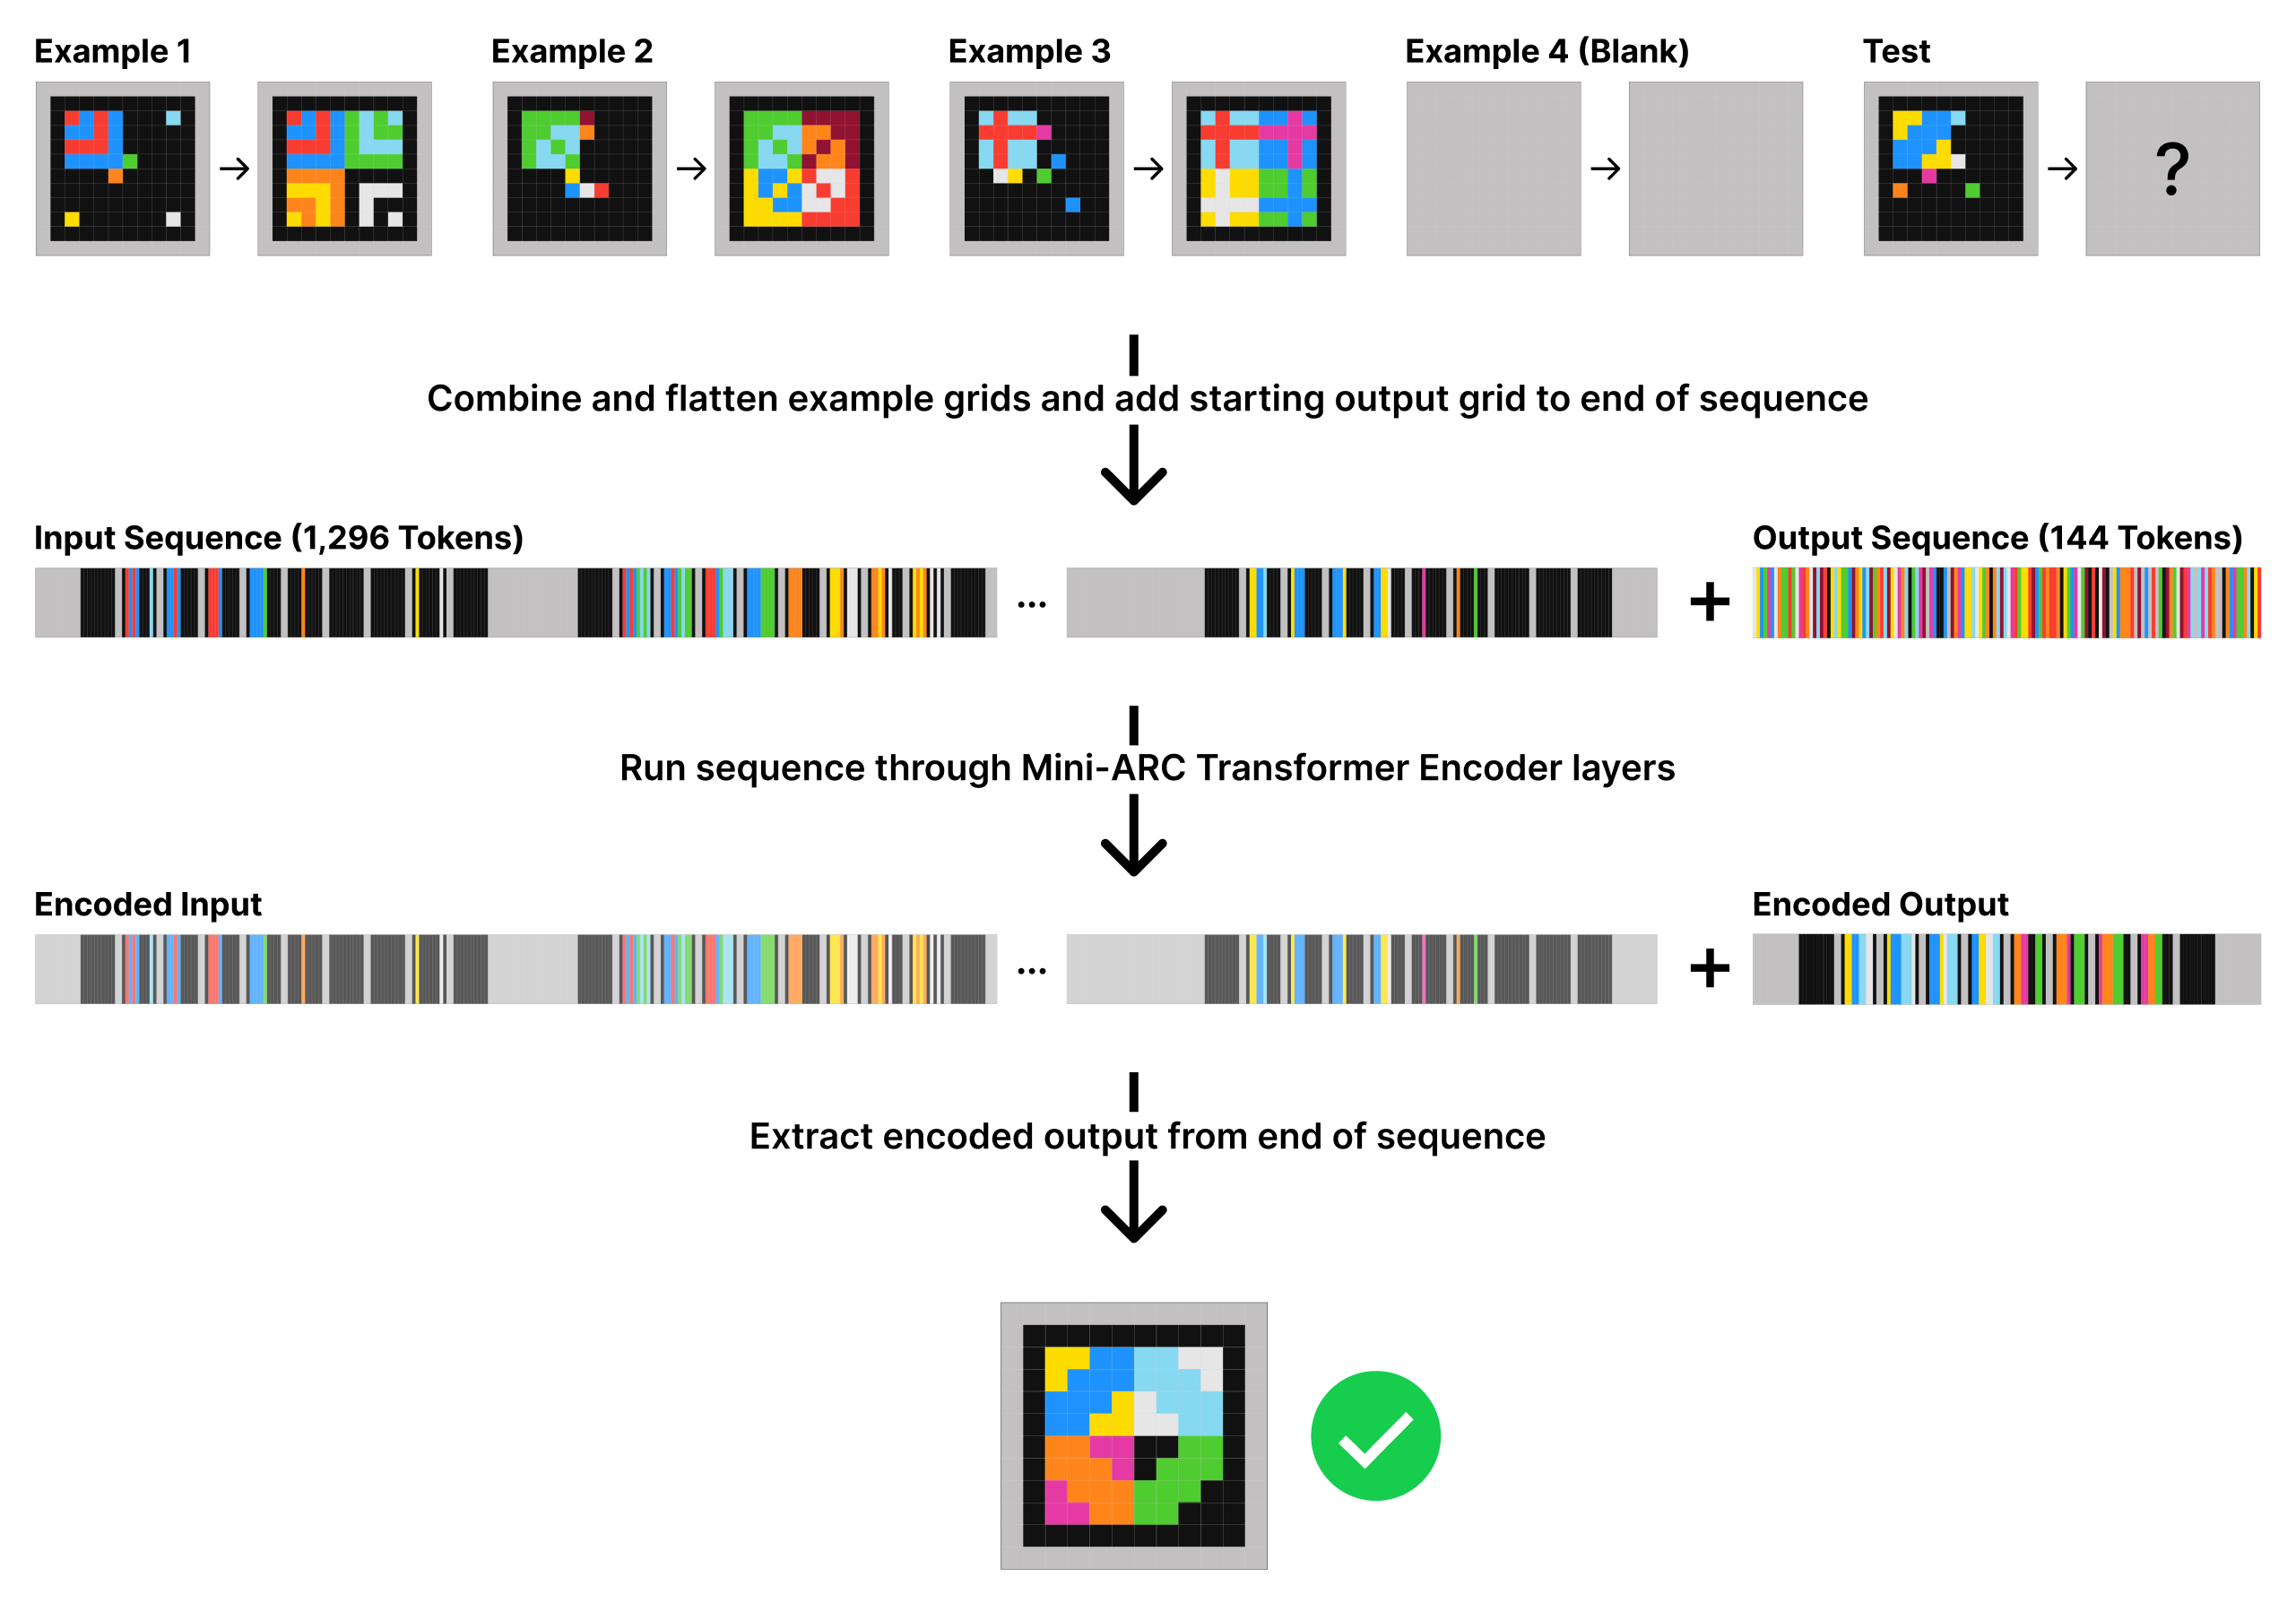
\includegraphics[width=\textwidth]{figures/sequence.png}
  \caption{Here is an illustration of how ARC Puzzle cfb2ce5a is
    encoded into a sequence along with a placeholder output grid and
  passed through the Mini-ARC model.}
  \label{fig:sequence-fig}
\end{figure*}

\subsection{Model Architecture}

At the core of Mini-ARC is a specialized Transformer model designed
for processing ARC puzzles. The model consists of:
\begin{enumerate}
  \item An embedding layer to convert discrete colors to vectors
  \item A custom positional encoding scheme that represents a cell's
    2-D position as well as it's position in the larger context
  \item A stack of Transformer self-attention encoder layers
  \item A final layer to project the output back to discrete colors
\end{enumerate}

I trained two models for evaluation: \textbf{Mini-ARC-12} and
\textbf{Mini-ARC-v12}. See Table 1 for the specifications and
hyperparameters used for each model. The only difference between the
two is that Mini-ARC-v12 uses a modified embedding scheme which
compresses each 12x12 grid into a 6x6 grid using 2x2
patches\cite{dosovitskiy2021imageworth16x16words}, which
is a common technique for Vision Transformers—thus the "v" in the
model name. Therefore, the input sequence for
Mini-ARC-v12 is considerably shorter than the un-patched input
sequence for Mini-ARC-12.

\begin{table}
  \centering
  \caption{Model Hyperparameters}
  \begin{tabular}{lccc}
    \toprule
    \textbf{\footnotesize{Specification}} &
    \textbf{\footnotesize{Mini-ARC-12}} &
    \textbf{\footnotesize{Mini-ARC-v12}} \\
    \midrule
    Max grid dim. & 12x12 & 12x12 \\
    Total parameters & 67,320,715 & 67,343,755  \\
    Sequence len. & 1,440 & 468 \\
    Embedding dim. & 512 & 512  \\
    FFN dim. & 3,072 & 3,072 \\
    Encoder layers & 16 & 16  \\
    Attention heads & 16 & 16 \\
    \bottomrule
  \end{tabular}
  \label{tab:model-specs}
\end{table}

\subsubsection{Input Representation}

In order to maximize in-context learning, an entire puzzle, including
all training input and output grids as well as the test input grid,
is included in the input.

While ARC puzzles have many context pairs and grids can be from 1x1
to 30x30, I chose to limit the sequence length for the sake of
more efficient experimentation. Mini-ARC-12 and Mini-ARC-v12 expect the input
to be nine 12x12 grids: four input and output train grids and one
test input grid.

All grids are padded to 12x12 using a padding token (0) and all
missing training pairs are padded with 12x12 grids as well. Since the
padding token is 0, the color classes are all bumped up by one before
being encoded.

The input tokens are flattened to make an input sequence of all nine
grids and a 12x12 output grid is added to the end. By default the
placeholder output grid is a learned parameter, but the models also
accept a custom starting output grid as an argument to the forward
pass. See Figure 2 for an illustration of how the full sequence is
constructed and Table 1 for the specific sequence lengths for each model.

\subsubsection{Embedding and Positional Encoding}
The sequence is embedded into 512-dimensional space using a
learned embedding parameter. Each token is augmented with a
positional encoding that includes: (1) its grid row, (2) its grid
column, (3) whether its part of an input or output grid, and (4)
which grid pair its a part of. The model has a learned embedding for
each of those four attributes.

\subsubsection{Attention and Masking}
The full embedded sequence is passed through 16 Transformer encoder
layers with self-attention mechanisms. A padding mask prevents
padding tokens from attending to other tokens. And a causal attention
mask prevents the input sequence from attending to the output
sequence. Input tokens can attend to any tokens in the input
sequence, and output tokens can attend to all tokens—both the input and output.

\subsection{Training Data and Synthetic Data Generation}

The ARC benchmark includes two datasets: the Public Training Set with
400 easy puzzles and the Public Evaluation Set with 400 hard puzzles.
While the point of the ARC Prize is to focus on generalization, I
needed more data in order to train the Mini-ARC models.

I ended up with a training dataset of 830,648 puzzles and an
evaluation dataset of 167,880 puzzles. All of these puzzles have 4 or
fewer training pairs and do not include any grids larger than 12x12.
While the ARC public datasets differ in complexity, the training and
evaluation datasets I used for
training are the same difficulty and complexity. The evaluation
dataset is just a random subset of the total dataset that was kept
out of training.

The dataset is a combination of three sources:
\begin{enumerate}
  \item 290,025 RE-ARC puzzles, which represent the 400 patterns and
    transformations from the ARC Public Training Set
  \item 524,506 BARC puzzles, which represent 200,000 patterns and
    transformations from the BARC Heavy dataset
  \item 16,117 ARC-HTML puzzles, which represent 30 patterns and
    transformations from the ARC Public Evaluation Set
\end{enumerate}

\subsubsection{ARC-HTML}

\begin{figure*}[h!]
  \centering
  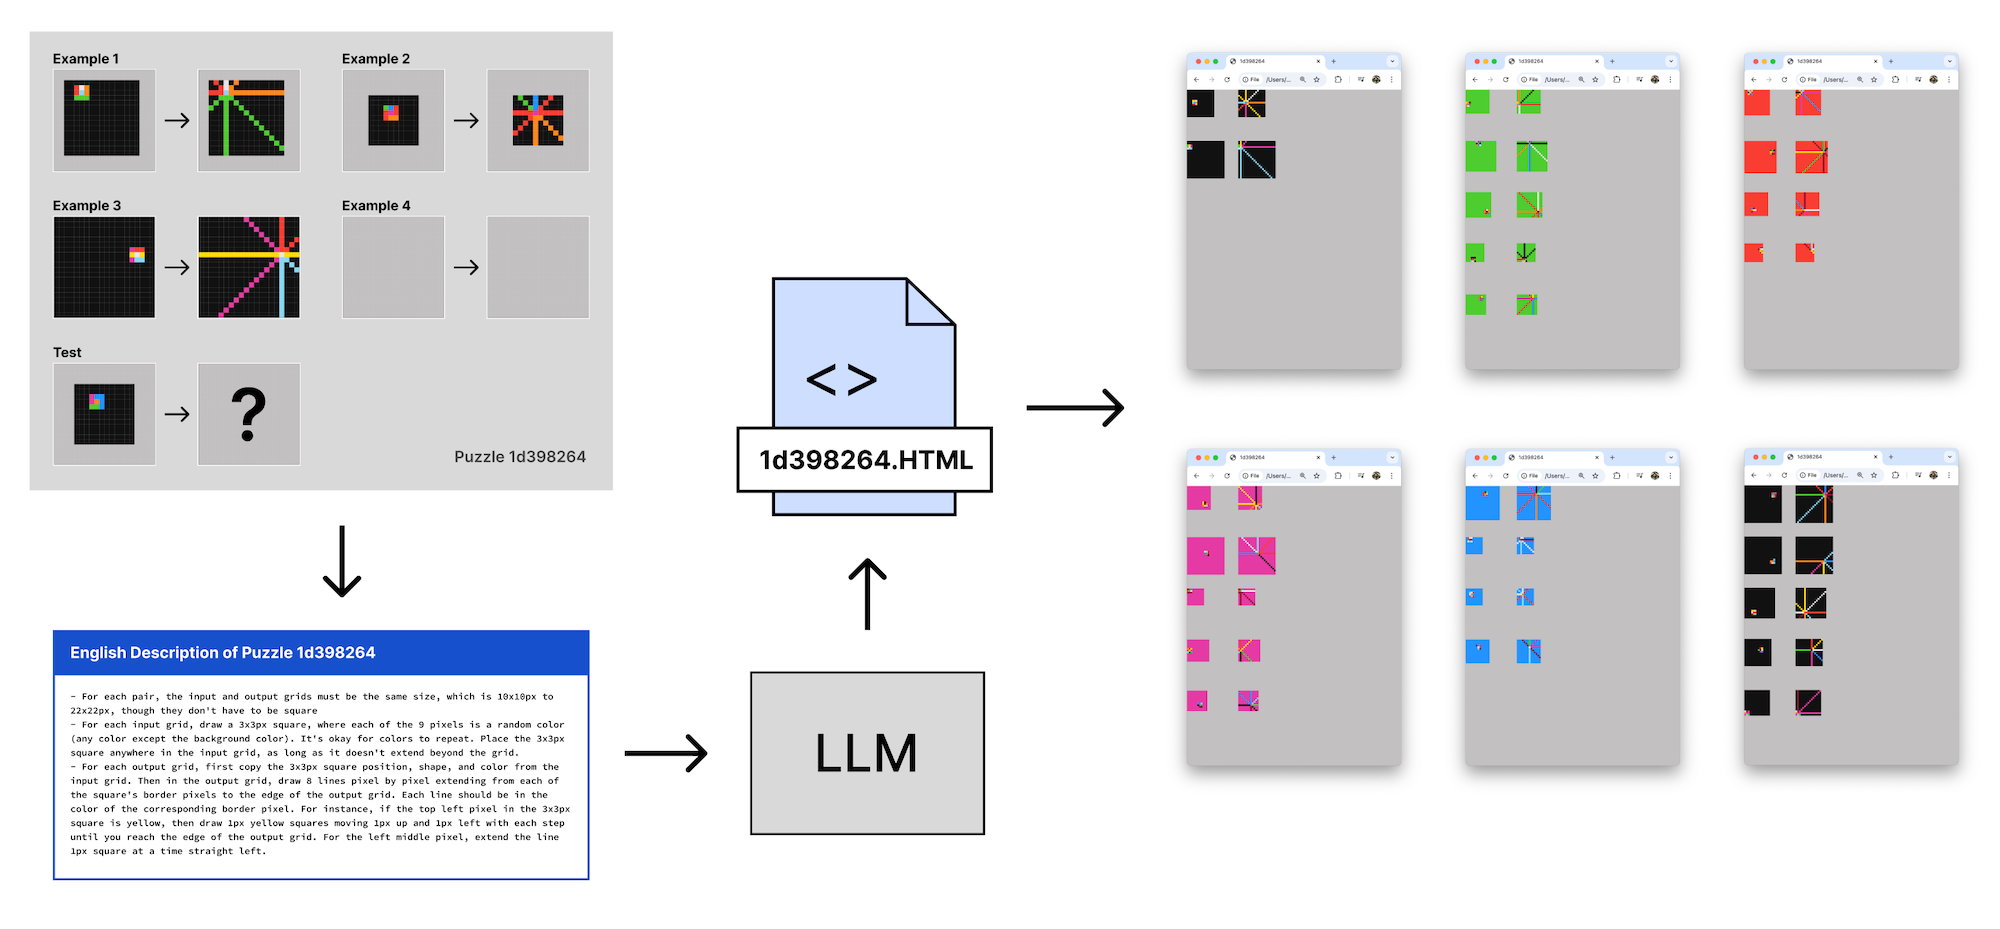
\includegraphics[width=\textwidth]{figures/html.png}
  \caption{ARC-HTML is a prompting strategy for getting LLMs to
  generate HTML documents where each page load yields a new ARC puzzle.}
  \label{fig:html}
\end{figure*}

In addition to the RE-ARC and BARC puzzles, I wanted to generate
puzzles similar in complexity to the ARC Evaluation Set. I initially
tried writing Python functions for each puzzle in the
ARC Public Evaluation Set, but that proved extremely tedious. I then
wrote out descriptions of some of the transformations represented in
the puzzles in English and tried prompting LLMs to
write Python programs for me. I even provided the RE-ARC DSL to LLMs
and tried having them use that. None of the Python-based approaches
proved successful or efficient. Either the
LLM-generated programs required heavy edits or they didn't work at all.

Eventually, I tried prompting LLMs to generate HTML
documents for each puzzle. I thought that the transformations and
patterns included in the puzzles might be easier for LLMs to write
with HTML, CSS, and Javascript, because they're often projections of
3D objects in a 2D space, similar to HTML pages. While it was still
burdensome to write English descriptions of the puzzles, I wrote 40
descriptions and ChatGPT and Claude wrote extensive HTML documents
for each one. I prompted them with a sample HTML document including
containers for the input/output grids. Then I wrote a script to load
each HTML document, take an image of the webpage, and parse it
pixel-by-pixel to turn each into ARC puzzles. Specific prompts
ensured that the HTML documents kept the grids at certain sizes so
that I could scrape them consistently.

From the 40 HTML documents, I generated 360,000 puzzles. Though only
16,117 of those from 30 HTML documents fit inside the 12x12 grid
limitation I imposed for training Mini-ARC. The 40
\href{https://github.com/pfletcherhill/mini-arc/tree/main/html}{HTML
documents}
and
\href{https://github.com/pfletcherhill/mini-arc/tree/main/prompts}{prompts} are
available on Github.

\subsection{Training}

Training of the Mini-ARC models was done using supervised learning on
4-8 A100 GPUs on Modal\cite{modal}
over multiple days. Both Mini-ARC-12 and Mini-ARC-v12 were trained
for at least 150,000 steps with effective batch sizes ranging from 32 to 192.

\subsection{Test-Time Training}

In addition to the pre-trained models, I also set up a test-time
training scheme where models could be fine-tuned for each individual
puzzle as they solve it. For each puzzle, I created a new dataset by
sampling pairs from the context input and output grid pairs in the
puzzle. So a puzzle with 4 context pairs would generate 48
fine-tuning puzzles by taking all the permutations of every
combination of at least 3 puzzles from the group.

At test time, I train a copy of the pre-trained model on the
puzzle-specific dataset using supervised learning. Training proceeds
until either an accuracy cut-off is achieved (typically 99\%) or a
number of steps is exceeded. The batch size, learning rate, number of
steps, and accuracy cut-off are all tunable arguments.

\subsection{Refinement}

The Mini-ARC models were trained with two settings: predicting from
scratch and refinement. The forward pass of the models accepts an
optional output argument, which if present will be used as the
starting point for the output grid. If no output argument is passed,
the output grid is set from a learned parameter on the model.

During training, I set 25\% of the training steps to focus on
refinement. In those steps, I generated a partial solution to the
puzzle and fed it into the model along with the input. Partial
solutions were created by adding varying amounts of noise to the real
outputs. The aim was to be able to refine a puzzle solution over
multiple passes.

\section{Results}

I evaluated each Mini-ARC model and strategy against a representative
subset of the public ARC Evaluation Dataset. This version of Mini-ARC models
is limited to puzzles with grids up to 12x12 in size and up to 4
pairs of training pairs. Therefore, I tested against a subset of the
public evaluation dataset that fit that criteria, which was 114
puzzles of the 400 available. See
Appendix~\ref{app:evaluation-dataset} for a list of all 114 puzzle IDs.

I used three metrics to evaluate each model:

\begin{enumerate}
  \item Score - how many of the puzzles did the model
    predict correctly?
  \item Accuracy - how many pixels did the model predict correctly?
  \item Closeness - how many of the puzzles did the model predict
    within 95\% accuracy?
\end{enumerate}

Each model was evaluated using three strategies:
\begin{enumerate}
  \item Zero-shot prediction
  \item TTT prediction - TTT for up to 15 epochs with accuracy cut-off of 99.5\%
  \item TTT + Refined prediction - TTT for up to 15 epochs, then 2
    rounds of refinement
\end{enumerate}

\begin{table*}
  \centering
  \caption{Mini-ARC Performance}
  \begin{tabular}{lccc}
    \toprule
    \textbf{Metric} & \textbf{Mini-ARC-12} &
    \textbf{Mini-ARC-v12} \\
    \midrule
    Zero-shot Score & 26 (22.8\%) & 11 (9.6\%)  \\
    Zero-shot Accuracy & 93.0\% & 90.7\%  \\
    Zero-shot Closeness & 56 (49.1\%) & 44 (38.6\%)  \\
    \addlinespace
    \cmidrule{1-3}
    TTT Score & 43 (37.7\%) & 17 (14.9\%)  \\
    TTT Accuracy & 95.0\% & 93.1\%  \\
    TTT Closeness & 78 (68.4\%) & 65 (57.0\%) \\
    \addlinespace
    \cmidrule{1-3}
    TTT + Refined Score  & \textbf{47 (41.2\%)} & 20 (17.5\%)  \\
    TTT + Refined Accuracy  & 95.3\% & 93.3\%  \\
    TTT + Refined Closeness  & 80 (70.2\%) & 64 (56.1\%)  \\
    \bottomrule
  \end{tabular}
  \label{tab:performance}
\end{table*}

As you can see in Table~\ref{tab:performance}, ARC-Mini-12 performs
significantly better than ARC-Mini-v12 in all
categories. 90\%+ accuracy was achieved by all strategies, which is
impressive, especially for the zero-shot predictions. Though keep in
mind that accuracy calculations include padding tokens in the output
grids. Assuming padding tokens are easier to predict than other
tokens, this accuracy calculation favors puzzles with small output
grids. The combination of test-time training and refinement achieves
the best result, solving 41.2\% of puzzles in the dataset.

\section{Discussion}
\subsection{Data Leakage}
Because the ARC-HTML portion of the Mini-ARC training dataset was
derived from puzzles in the ARC Public Evaluation Set, there is a
concern about data leakage when benchmarking
performance against the ARC Public Evaluation Set. However, the
overlap between the puzzles used to generate the ARC-HTML dataset and
the puzzles in the 114 limited evaluation dataset is only 10 puzzles.
I did not consider grid sizes when picking puzzles for the
ARC-HTML dataset, and many of them exceed the 12x12 grid constraint
for training Mini-ARC-12 and Mini-ARC-v12.

Across the 10 puzzles that do overlap, the Mini-ARC performance is
similar to the rest
of the evaluation dataset, solving a maximum of 4 of the 10 puzzles
in any of the performance metrics. See a full report of the results
on these 10 puzzles in Appendix~\ref{app:leakage-results}.

\subsection{Limitations}
One limitation of a system like Mini-ARC compared to
strategies that use LLMs is that Mini-ARC has to handle both
reasoning and program execution, while LLMs are able to write code to
test their programs and offload computation to a computer. The
combination of these modes in Mini-ARC is similar to
humans—we are able to execute the transformations we contemplate
mentally without having to write Python programs to try them—but it
is still a disadvantage relative to other approaches.

\subsection{Future Work and Other Ideas}
\subsubsection{Scale Up Models to Larger Grids}
The current Mini-ARC models are constrained by their 12x12 grid size
requirement. In the future, I would like to train larger models with
the same architecture to evaluate against larger ARC puzzles. While
Mini-ARC-12 performed better than Mini-ARC-v12 at this size, using
Vision Transformer-style patch embedding will be important as we
scale up to keep the sequence length reasonable. Without using
patches, the sequence length for 30x30 puzzles would be 9,000 tokens,
which would require a much larger model.
For comparison, the current context window for OpenAI's GPT-3.5 is
16,385 tokens.

\subsubsection{ARC-HTML Experimentation}
The ARC-HTML approach demonstrated that advanced LLMs are capable of
formalizing ARC puzzles in HTML, CSS, and Javascript documents.
In addition to prompting LLMs to follow instructions for specific
puzzles, we should try prompting them to generate HTML documents for
new puzzles entirely. This strategy is similar to BARC\cite{barc},
which cleverly prompted LLMs to generate new puzzles from seed
programs, where the seed programs represented a diverse set of grid
transformations. But since ARC-HTML puzzles are HTML documents, in
order to get an even more diverse dataset, we could prompt LLMs to
modify ARC-HTML puzzles using all possible CSS transformations.

\subsubsection{Meta Learning}
Since test-time training has proven to be effective, future work
should be done to evaluate meta learning strategies\cite{maml}.
Currently, training and test-time training occur independently, but
theoretically we should be trying to minimize the loss after
test-time training rather than zero-shot prediction, which may result in a
different state for the model parameters.

\section{Conclusion}
This paper introduces Mini-ARC, a collection of small Transformer models
trained on ARC puzzles as well as test-time training (TTT) and refinement
strategies for solving ARC puzzles. Using Mini-ARC-12, I show a best
performance of 41\%
across a subset of the ARC evaluation dataset, which is filtered to
puzzles that fit the Mini-ARC grid size constraints. This result is
notable because of the relatively small
size of the models (67M params) and because it was achieved without
the use of language models, search, or program synthesis.

\bibliographystyle{plain}
\bibliography{references}

\appendix

\section{Mini-ARC Evaluation Dataset}
\label{app:evaluation-dataset}

Here are the 114 puzzles from the public ARC Evaluation Set that fit
within the Mini-ARC size constraints: 3b4c2228, fc754716, 5d2a5c43,
e5790162, 4e469f39, 6ea4a07e, bf32578f, ef26cbf6, ca8de6ea, 5783df64,
9c56f360, d017b73f, 626c0bcc, c35c1b4c, c48954c1, b15fca0b, 4acc7107,
ac605cbb, f0afb749, c8b7cc0f, da2b0fe3, ae58858e, e99362f0, 67c52801,
66e6c45b, 48131b3c, 2685904e, 90347967, a406ac07, 60c09cac, 332efdb3,
b1fc8b8e, 506d28a5, dc2aa30b, 8fbca751, 17cae0c1, e633a9e5, ed74f2f2,
ecaa0ec1, 68b67ca3, f45f5ca7, cfb2ce5a, 7ee1c6ea, 48f8583b, aa300dc3,
9f27f097, 4cd1b7b2, 31adaf00, e345f17b, 2072aba6, 9c1e755f, f3e62deb,
c7d4e6ad, a8610ef7, 84db8fc4, 31d5ba1a, 7953d61e, bbb1b8b6, 0692e18c,
782b5218, 0c786b71, 575b1a71, 2c737e39, 94414823, 137f0df0, 6f473927,
00576224, a59b95c0, b942fd60, 4852f2fa, 6ad5bdfd, d19f7514, 8b28cd80,
27f8ce4f, ea9794b1, 73182012, 917bccba, d2acf2cb, 8e2edd66, e5c44e8f,
ce039d91, 15696249, f3cdc58f, 73c3b0d8, 34b99a2b, b0722778, e7dd8335,
1acc24af, e133d23d, 69889d6e, 9110e3c5, 12eac192, c074846d, 64a7c07e,
8ba14f53, e872b94a, e6de6e8f, 85fa5666, 8597cfd7, 7e02026e, 32e9702f,
59341089, 03560426, 3979b1a8, aa18de87, af24b4cc, e69241bd, be03b35f,
27a77e38, 0becf7df, 3d31c5b3, 7c8af763, 6df30ad6, ed98d772.

\section{ARC-HTML Prompt}
Here is an example prompt used for generating HTML files from English
descriptions of ARC puzzles via LLMs:

\begin{lstlisting}
  Update this HTML document using the instructions below. Think step-by-step and make sure the HTML is correct. The name of the puzzle is <Insert Puzzle ID>.

  <Insert HTML template here>

  General Instructions:
  - Change the HTML title to the name of the puzzle
  - On each page load, pick a random number of pairs (between 2-5) and add more pairs using the pattern already in the document for the first two pairs. The number of pairs should be determined randomly with each page load.
  - Each pair should include two containers, sized 30x30 pixels each. Each container will contain an input grid div and an output grid div, which the puzzle instructions will help you define. Do not change the size of the containers, only the sizes of the grids inside them.
  - Do not modify the CSS for main, pair, container classes. None of the classes in the template should be changed.
  - Pick a background color for all the grids, which should be black for 60% of puzzles

  Instructions for puzzle <Insert Puzzle ID>:
  <Insert Puzzle Description>

  Warnings:
  - Do not use a canvas, because the output will be blurry.
  - Make sure your script does not cause an infinite loop or cause the page to crash when the HTML is loaded.
  - Just return the HTML document for saving in a file.

\end{lstlisting}

\section{ARC-HTML Data Leakage Investigation Results}
\label{app:leakage-results}

The 10 puzzles that are both in the 114 Mini-ARC evaluation dataset
and the ARC-HTML 12x12 training dataset are: 0becf7df, 00576224,
0c786b71, 03560426, 137f0df0, 17cae0c1, 12eac192, 15696249, 332efdb3,
32e9702f. See Table~\ref{tab:leakage-performance} for performance on
these 10 puzzles.

\begin{table}[h]
  \centering
  \caption{Mini-ARC Data Leakage Puzzle Performance}
  \begin{tabular}{lccc}
    \toprule
    \textbf{\footnotesize{Metric}} & \textbf{\footnotesize{Mini-ARC-12}} &
    \textbf{\footnotesize{Mini-ARC-v12}} \\
    \midrule
    \small{Zero-shot Score} & 3 (30.0\%) & 2 (20.0\%)  \\
    \small{Zero-shot Accuracy} & 93.0\% & 91.1\%  \\
    \small{Zero-shot Closeness} & 5 (50.0\%) & 3 (30.0\%)  \\
    \addlinespace
    \cmidrule{1-3}
    \small{TTT Score} & 4 (40.0\%) & 3 (30.0\%)  \\
    \small{TTT Accuracy} & 91.2\% & 94.7\%  \\
    \small{TTT Closeness} & 5 (50.0\%) & 5 (50.0\%) \\
    \addlinespace
    \cmidrule{1-3}
    \small{TTT + Refined Score} & 4 (40.0\%) & 3 (30.0\%)  \\
    \small{TTT + Refined Accuracy} & 91.7\% & 94.9\%  \\
    \small{TTT + Refined Closeness} & 5 (50.0\%) & 5 (50.0\%)  \\
    \bottomrule
  \end{tabular}
  \label{tab:leakage-performance}
\end{table}

\end{document}
